\section{Aula 3}

\subsection{Método Newton-Raphson}
O Método Newton-Raphson tem como objetivo estimar as raízes de uma
função, escolhendo uma aproximação inicial para esta e após a escolha
calcular a equação tangente da função neste ponto e a interseção dela
com o eixo das abcissas, a fim de encontrar uma melhor aproximação
para a raiz. O processo é repetido, criando assim um método iterativo
para encontrar a raiz da função. O algoritmo para o caso univariado é apresentado a seguir.


\begin{framed} %Box algoritmo
    \textbf{O algoritmo de Newton-Raphson}
    
    \begin{enumerate}
    \item Arbitrar uma condição inicial $(x_{i}-x_{0})$ e fixar $i=0$;
    
    \item Calcular $f(x_{i})$ e verificar a convergência. Se $|f(x_{i})|\leq \varepsilon$, então parar.
    
    \item Linearizar a função em torno de $(f(x_{i}),x_{i})$ e igualar a função
    a zero para estabelecer o passo $(\triangle x_{i}=x_{i+1}-x_{i})$
    e novo ponto $(x_{i+1})$.
    $$f(x)=f(x_{i})+f^{'}(x_{i})\cdot(x_{i+1}-x_{i})=0$$
    $$x_{i+1}=x_{i}-\frac{f(x_{i})}{f^{'}(x_{i})}$$
    
    \item Fazer $i=i+1$e voltar ao passo 2.
    
    \end{enumerate}
    
    Uma representação  gráfica do algoritmo é mostrada na figura \ref{fig:aula3_7}.
    
\end{framed}

\begin{figure}[H]
\begin{centering}
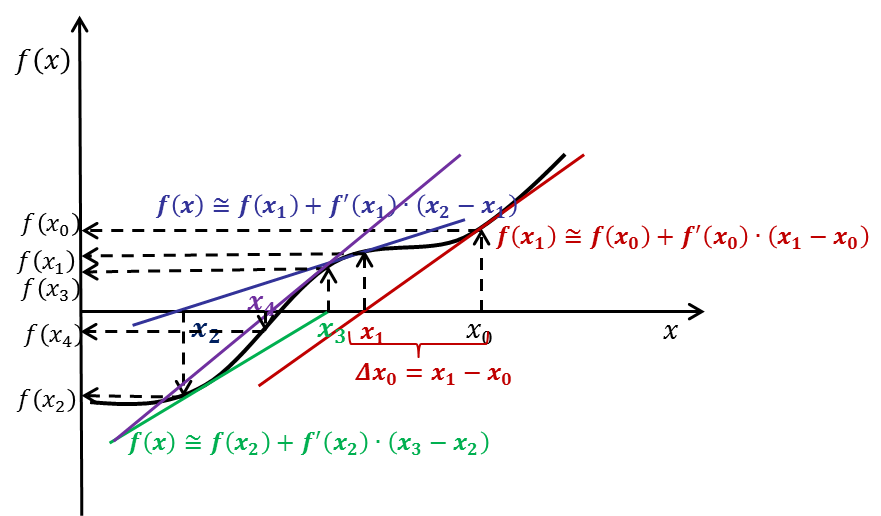
\includegraphics[scale=0.8]{aula3_7}\protect\caption{\label{fig:aula3_7} Algoritmo do Método de Newton  }
\end{centering}
\end{figure}

O método de Newton se baseia na expansão por \textbf{séries de Taylor} que, por definição, é uma forma de aproximar uma função $f$ ao redor de um ponto $x_{0}$ através da soma de polinômios.
Se uma função e suas derivadas até a ordem $n+1$ forem contínuas
em um intervalo contendo $x$ e $x_{0}$, então a expansão de Taylor é dada por: 

\[
f(x)=f(x_{0})+f^{'}(x_{0})\cdot(x-x_{0})+\frac{1}{2!}\cdot f^{''}(x_{0})\cdot(x-x_{0})^{2}+...+\frac{1}{n!}\cdot f^{(n)}(x_{0})\cdot(x-x_{0})^{n}+R_{n}.
\]

A representação gráfica dos termos da série de Taylor é dada pela Figura \ref{fig:aula3_2}.

\begin{figure}[H]
\begin{centering}
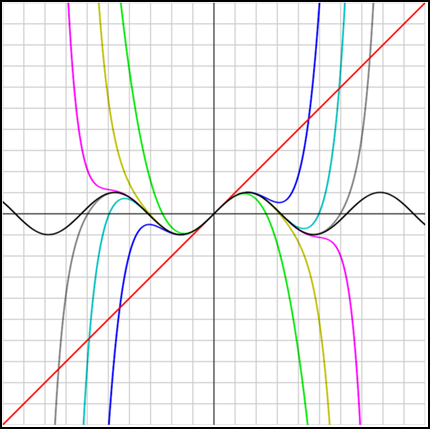
\includegraphics{aula3_2}\protect\caption{\label{fig:aula3_2} Série de Taylor }
\end{centering}
\end{figure}


Truncando a série no termo de 1ª ordem (ou seja, descartando todos os termos de ordem superior a 2), temos: 
\[
	f(x)=f(x_{0})+f^{'}(x_{0})\cdot(x-x_{0}).
\]
Tomando a expansão em torno de $x_0$, a interseção desta reta com o eixo das abcissas é encontrada em $x'$ resolvendo a equação: 
\[
	x' = x_0 - \dfrac{f(x_0)}{f'(x_0)} .
\]
Assim, o algoritmo funciona tomando o $x'$ como o valor de $x_{i+1}$ depois da $i$-ésima iteração, e continuando o algoritmo até atender um critério de parada. 
%  Como queremos (escolha inicial):
%\[
%x_{1}=x_{0}-\frac{f(x_{0})}{f^{'}(x_{0})},
%\]


\begin{exemplo}
Seja a função $f(x)=x^{2}-6\cdot\sin(x)$ com $x\in[1;3]$. Uma maneira de se encontrar a solução é plotar a função e procurar a solução visualmente, conforme na figura \ref{fig:aula3_1}. 
\begin{figure}[H]
\begin{centering}
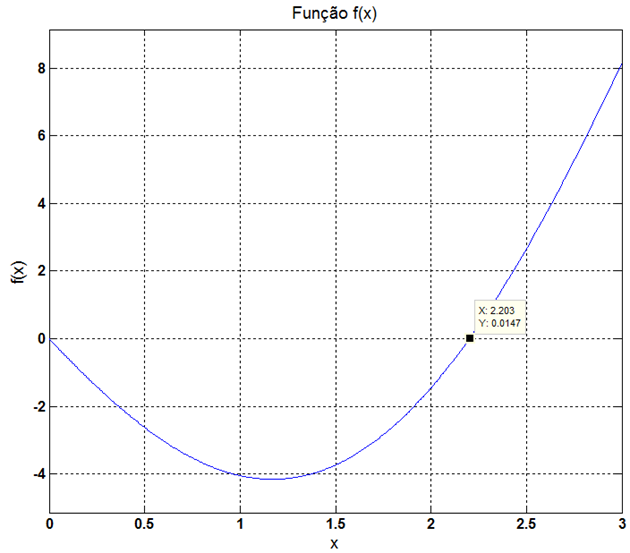
\includegraphics{aula3_1}\protect\caption{\label{fig:aula3_1} Solução gráfica }
\end{centering}
\end{figure}

Considerando
uma escolha inicial de $x_{0}=2,5$, vamos utilizar o método de Newton-Raphson para aproximar uma raiz da função $f$ com uma tolerância $\varepsilon=0,05$.  Para a primeira iteração, devemos procurar
\[
x_{1}=x_{0}-\frac{f(x_{0})}{f^{'}(x_{0})},
\]
A função avaliada em $x_{0}=2,5$, com as derivadas em torno do ponto resultam
em:
\begin{eqnarray*}
f(x_{0}) & = & f(2,5)=2,6592 \\
f^{'}(x_{0}) & = & f^{'}(2,5)=9,8069
\end{eqnarray*}
Assim, substituindo os valores na equação para $x_{0}=2,5$, obtém-se uma aproximação da função $f$ em torno de $x_0$:
\[
f(x)\cong2,66+9,81\cdot(x-2,5).
\]

\begin{figure}[H]
\begin{centering}
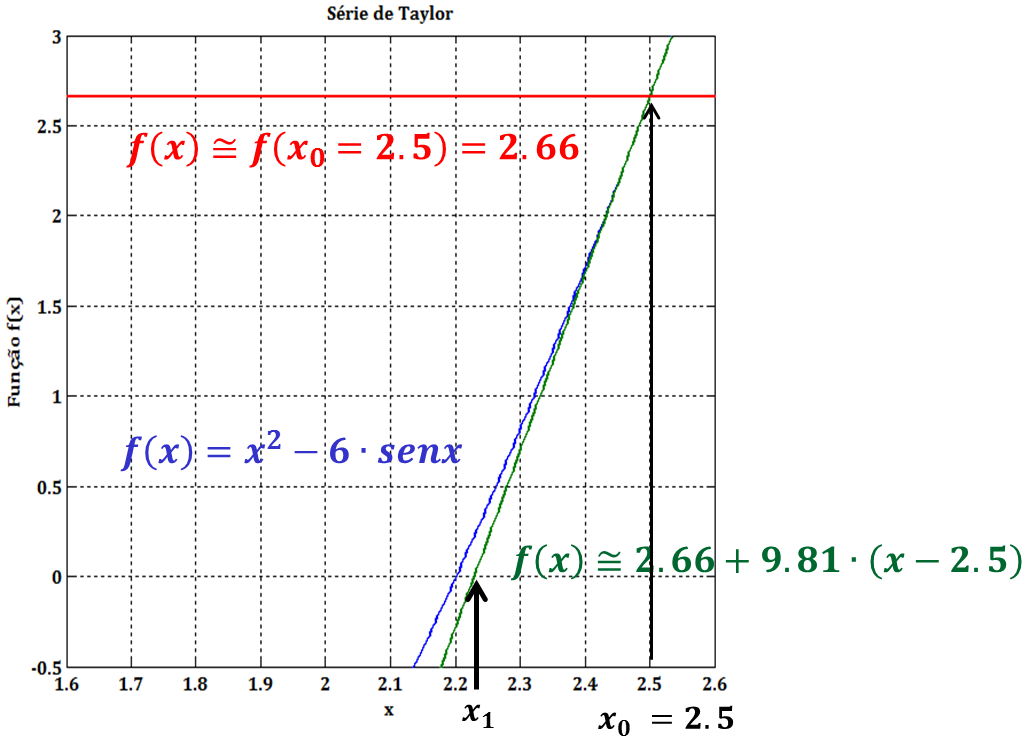
\includegraphics[scale=0.8]{aula3_3}\protect\caption{\label{fig:aula3_3} Gráfico  $x_{0}=2,5$  }
\end{centering}
\end{figure}
Na figura \ref{fig:aula3_3}, a reta azul representa a função original do problema e a verde é a expansão em série de Taylor linearizada no polinômio de primeira ordem. O ponto $x_1$ é encontrado através da expressão
\[
x_{1}=2,5-\frac{2,6562}{9,8069}\cong2,23.
\]
Usando o ponto $x_{1}=2,23$ na função $f(x)=x^{2}-6\cdot\sin(x)$:

\[
| f(2,23)|=|2,23^{2}-6\cdot\sin(2,23)|=|0,23|>0,05
\]
A solução $x_{1}=2,23$ não satisfaz a restrição do problema. Utilizamos o $x_1$ para a próxima iteração (ver figura \ref{fig:aula3_4}), temos que 
\begin{figure}[H]
\begin{centering}
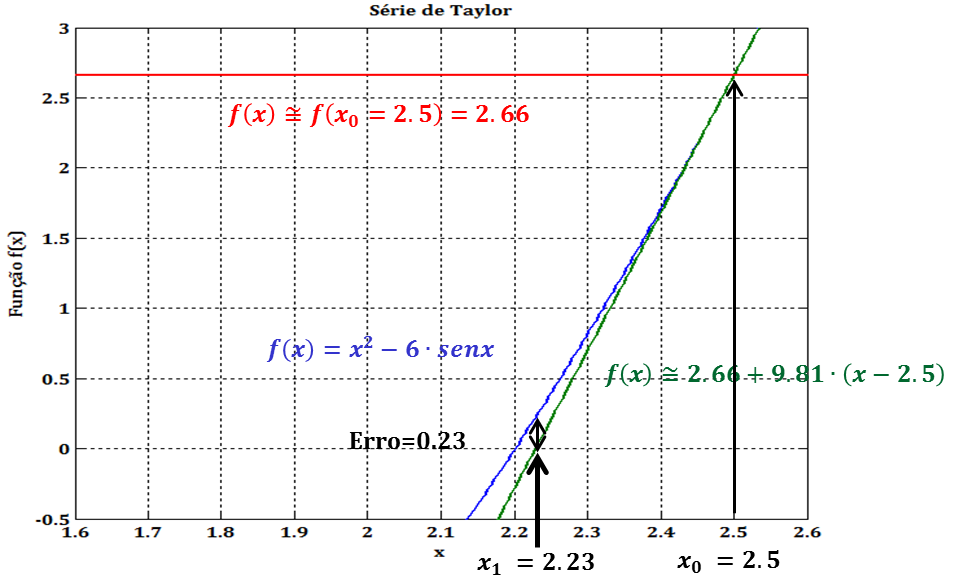
\includegraphics[scale=0.8]{aula3_4}\protect\caption{\label{fig:aula3_4} Gráfico com a tolerância de $x_{0}=2,5$  }
\end{centering}
\end{figure}
O ponto $x_{1}=2,23$ é o ponto de partida para a segunda iteração.
Linearizando em torno de $x_{1}=2,23$ (Gráfico \ref{fig:aula3_5}):
\begin{figure}[H]
\begin{centering}
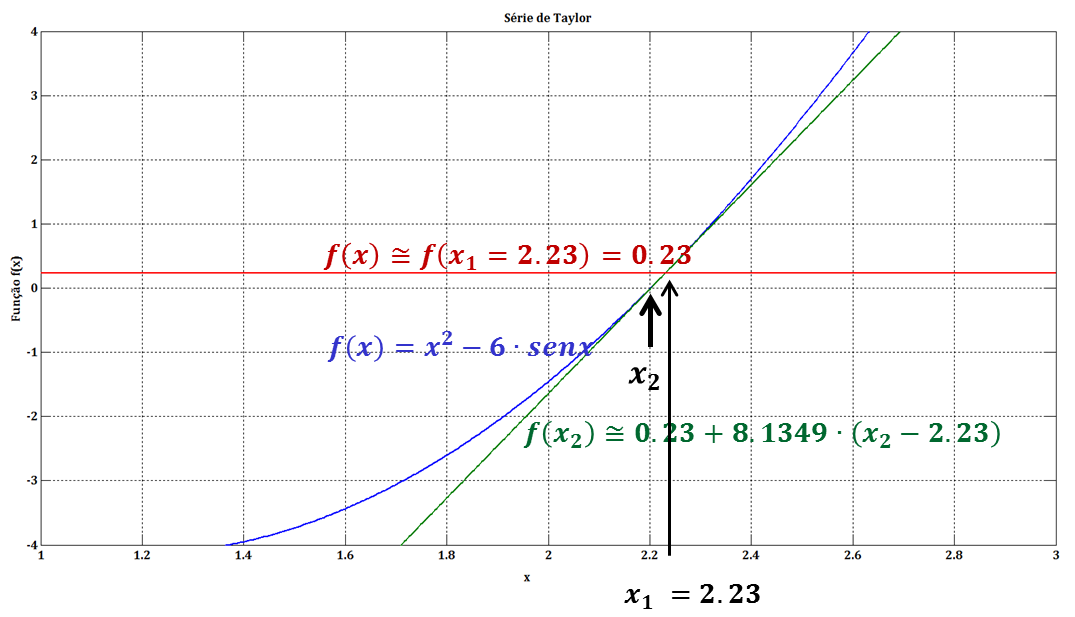
\includegraphics[scale=0.8]{aula3_5}\protect\caption{\label{fig:aula3_5} Linearização no ponto $x_{1}=2,23$  }
\end{centering}
\end{figure}
$$f(x_{1})=f(2,23)=0,23,$$
$$f^{'}(x_{1})=f^{'}(2,23)=8,1319,$$
$$x_{2}=x_{1}-\frac{f(x_{1})}{f^{'}(x_{1})}.$$
Assim, temos que:
$$f(x)\cong0,23+8,1349\cdot(x_{2}-2,23)$$
$$x_{2}=2,23 - \frac{0,23}{8,81349} \cong 2,20.$$
Usando o ponto $(x_{2}=2,2)$ na função $f(x_{2}^{2})=x_{2}^{2}-6\cdot\sin x_{2}$:
\[
	|f(2,2)|=|2,2^{2}-6\cdot\sin(2,2)|=|0,03|<0,05.
\]
Portanto, $x_{2}=2,2$ satisfaz a solução do problema. Caso seja necessário
encontrar uma tolerância menor que $0,03$ o processo deve ser repetido.
Graficamente, para $x_{1}=2,23$:
\begin{figure}[H]
\begin{centering}
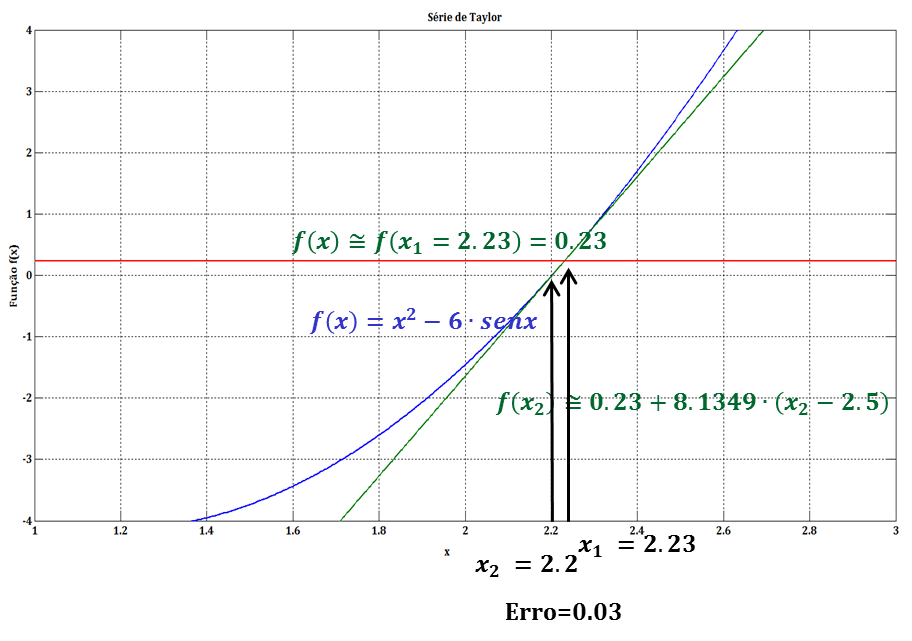
\includegraphics[scale=0.8]{aula3_6}\protect\caption{\label{fig:aula3_6} Gráfico para $x_{1}=2,23$  }
\end{centering}
\end{figure}







\begin{figure}[H]
\begin{centering}
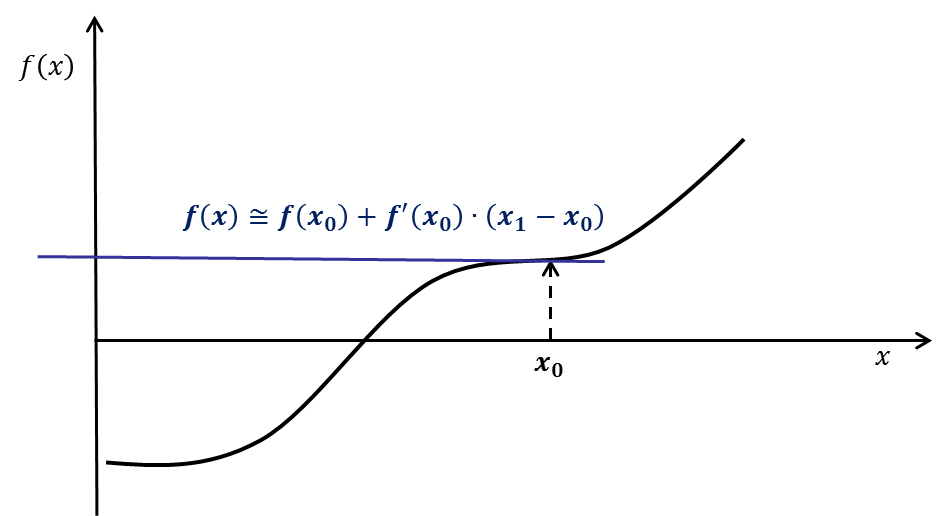
\includegraphics[scale=0.8]{aula3_8}\protect\caption{\label{fig:aula3_8} Escolha inicial  }
\end{centering}
\end{figure}

\end{exemplo}


Ao aplicar o método de Newton, deve-se tomar cuidado. O método é eficiente quando o ponto inicial $x_0$ é relativamente próximo da solução, mas pode ser ruim quando o chute inicial não for bom. Observe a figura \ref{fig:aula3_8}. A derivada avaliada em $x_0$ é 0, assim $x_{1}=x_{0}-\frac{f(x_{0})}{f^{'}(x_{0})}$; como o termo $\frac{f(x_{0})}{f^{'}(x_{0})}$ vai para infinito, a solução nunca seria encontrada. 

O método de Newton é adequado para o problema do fluxo de potência. Como as soluções do problema ($V$ e $\theta$) normalmente são próximas de 1 (um) pu e 0 (zero) radianos, então a escolha da solução inicial será normalmente adequada.

A diferença do fluxo de potencial do exemplo anterior é que temos
um conjunto de funções para resolver.

Já o \textbf{método de Newton aplicado ao caso multivariável} deve considerar:
\[
\begin{matrix} 
F(x)= & [f_{ 1 } & { f }_{ 2 } & ... & { f }_{ n }{ ] }^{ T } 
\end{matrix}
\begin{matrix} 
x= & [x_{ 1 } & { x }_{ 2 } & ... & { x }_{ n }{ ] }^{ T } 
\end{matrix}
\]
Sendo que, $F(x)$ representa um vetor de funções e $x$ é um conjunto
de variáveis.


\begin{framed} %Box algoritmo multivariado
    \textbf{O algoritmo de Newton-Raphson multivariado}
    \begin{enumerate}
    \item Arbitrar uma condição inicial $(x^{(i)}=x^{(0)})$ e fixar $i=0$;
    
    \item Calcular $F(x^{(i)})$ e verificar a convergência. Se $\max| F(x^{(i)})|\leq \varepsilon,$ então parar.
    
    \item Linearizar a função em torno de $(F(x^{(i)}),x^{(i)})$ e igualar
    a função a zero para estabelecer o passo $(\triangle x^{(i)}=x^{(i+1)}-x_{i}^{(i)})$
    e novo ponto $(x^{(i+1)})$.
    Para o caso de apenas uma variável, temos que:
    \[
    f(x)=f(x_{i})+f^{'}(x_{i})\cdot(x_{i+1}-x_{i})=0
    \]
    \[
    x_{i+1}=x_{i}-\frac{f(x_{i})}{f^{'}(x_{i})}.
    \]
    Já para o caso multivariado, temos que:
    \[
    F(x)=F(x^{(i)})+[J(x^{(i)})]\cdot(x^{(i+1)}-x^{(i)})=0
    \]
    \[
    x^{(i+1)}=x^{(i)}-[J(x^{(i)})]^{-1}\cdot F(x^{(i)}),
    \]
    sendo que $J(x^{(i)})=[\frac{\partial F(x)}{\partial x}]$ é a matriz jacobiana
    de derivadas de $F(x)$ com relação à $x$.
    \item Fazer $i=i+1$ e voltar ao passo 2.
    \end{enumerate}
    
    
\end{framed}


Para calcular a matriz jacobiana, primeiro cria-se um vetor $F$ com as $n$ funções em questão:
\[
\begin{matrix} 
F(x)= & [f_{ 1 } & { f }_{ 2 } & \dots & { f }_{ n }{ ] }^{ T }, 
\end{matrix}
\]
em que $\begin{matrix} 
x= & [x_{ 1 } & { x }_{ 2 } & \dots & { x }_{ n }{ ] }^{ T } 
\end{matrix}$. A matriz jacobiana é dada pelas derivadas cruzadas da função $F$:
\[
	\left[J(x^{(i)})\right]=\left[\frac{\partial F(x)}{\partial x}\right]=\left[\begin{array}{ccc}
	\frac{\partial f_{1}}{\partial x_{1}} & \cdots & \frac{\partial f_{1}}{\partial x_{m}}\\
	\vdots & \ddots & \vdots\\
	\frac{\partial f_{n}}{\partial x_{1}} & \vdots & \frac{\partial f_{n}}{\partial x_{m}}
	\end{array}\right]
\]
As equações básicas do subproblema 1 (barras PQ+PV) a serem solucionadas
são:
\[
P_{k}=V_{k}\sum_{m=1}^{n}V_{m}(G_{km}\cos\theta_{km}+B_{km}\sin\theta_{km}),\forall k\in\{\Omega_{PQ},\Omega_{PV}\},
\]
\[
Qk=V_{k}\sum_{m=1}^{n}V_{m}(G_{km}\sin\theta_{km}+B_{km}\cos\theta_{km}),\forall k\in\{\Omega_{PQ}\},
\]
onde, $\Omega_{PQ}$ são os conjuntos de barras do tipo PQ, $\Omega_{PV}$ são os conjuntos de barras do tipo PV. Considerando que para algumas barras os valores de P e Q são conhecidos, os ``resíduos'' de potência são dados por:
\[
\Delta P_{k}=P_{k}^{(especificado)}-P_{k}^{(calculado)}(V,\theta),\forall k\in\{\Omega_{PQ},\Omega_{PV}\},
\]
\[
\Delta Q_{k}=Q_{k}^{(especificado)}-Q_{k}^{(calculado)}(V,\theta),\forall k\in\{\Omega_{PQ}\},
\]
em que $P_{k}^{(especificado)}$ são os valores de potência ativa (conhecidos) na
barra $k$ e $Q_{k}^{(especificado)}$ são os valores de potência ativa(conhecido) na barra $k$.

Neste caso: \todo{como apresentar isso aqui?}
\[
	\begin{matrix}
	F(\Delta { P },\Delta Q)= & [\Delta { P }_{ 1 } & \Delta { P }_{ 2 } & ... & \Delta { P }_{ n }^{ \quad } & \Delta { Q }_{ 1 } & \Delta { Q }_{ 2 } & \dots & { \Delta { Q } }_{ n }] 
	\end{matrix}
\]
\[
	\begin{matrix} 
	x= & [\theta _{ 1 } & \theta _{ 2 } & ... & \theta _{ n }^{ \quad } & V_{ 1 } & V_{ 2 } & \dots & { V }_{ n }] 
	\end{matrix}
\]

A matriz Jacobiana associada ao problema proposto é apresentada na Figura \ref{fig:aula3_9}.


\begin{figure}[H]
\begin{centering}
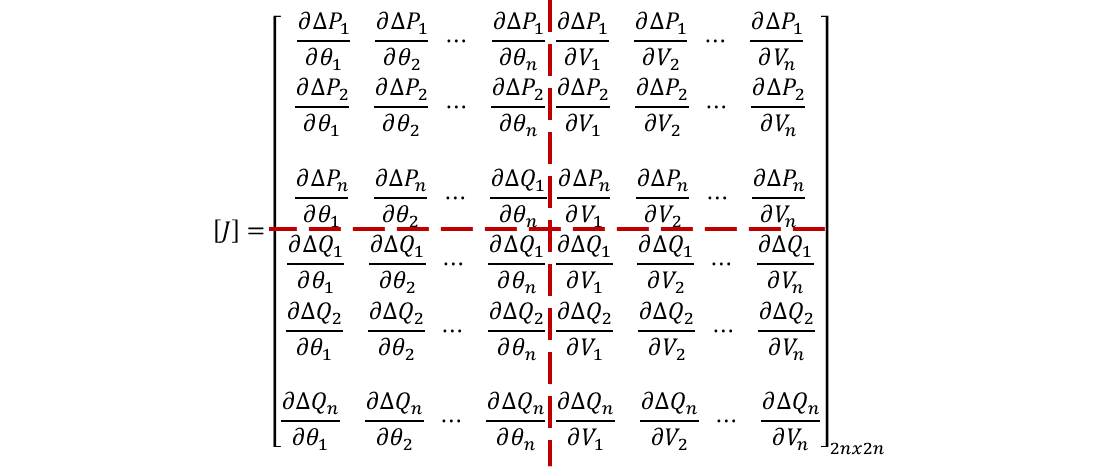
\includegraphics{aula3_9}\protect\caption{\label{fig:aula3_9} Matriz jacobiana  }
\end{centering}
\end{figure}

A seguir, calculamos os elementos da matriz jacobiana:
\[
\frac{\partial\triangle P_{k}}{\partial\theta_{m}}=\frac{\partial(P_{k}^{(especificado)}-P_{k}^{(calculado)})}{\partial\theta_{m}}=-\frac{\partial P_{k}^{(calculado)}}{\partial\theta_{m}},\qquad\forall m,k
\]
\[
\frac{\partial\triangle P_{k}}{\partial V_{m}}=\frac{\partial(P_{k}^{(especificado)}-P_{k}^{(calculado)})}{\partial V_{m}}=-\frac{\partial P_{k}^{(calculado)}}{\partial V_{m}},\qquad\forall m,k
\]
\[
\frac{\partial\triangle Q_{k}}{\partial\theta_{m}}=\frac{\partial(Q_{k}^{(especificado)}-Q_{k}^{(calculado)})}{\partial\theta_{m}}=-\frac{\partial Q_{k}^{(calculado)}}{\partial\theta_{m}},\qquad\forall m,k
\]
\[
\frac{\partial\triangle Q_{k}}{\partial V_{m}}=\frac{\partial(Q_{k}^{(especificado)}-Q_{k}^{(calculado)})}{\partial V_{m}}=-\frac{\partial Q_{k}^{(calculado)}}{\partial V_{m}},\qquad\forall m,k
\]


Como $P_{k}^{(especificado)}$ e
$Q_{k}^{(especificado)}$ são constantes a matriz Jacobiana pode ser reescrita como apresentamos a seguir:
\[
[J]=- \begin{bmatrix} \frac { \partial { P }^{ (calculado) } }{ \partial \theta } & \frac { \partial { P }^{ (calculado) } }{ \partial V } \\ \frac { \partial { Q }^{ (calculado) } }{ \partial \theta } & \frac { \partial { Q }^{ (calculado) } }{ \partial V } \end{bmatrix}_{ 2n \times 2n }=-{ \begin{bmatrix} H & N \\ M & L \end{bmatrix} }_{ 2n \times 2n }
\]
\[
H_{km}=\frac{\partial P_{k}^{(calculado)}}{\partial\theta_{m}}=V_{k}\cdot V_{m}\cdot\{G_{km}\cdot\sin(\theta_{km})-B_{km}\cdot\cos(\theta_{km})\},\forall k\neq m
\]


\[
H_{km}=\frac{\partial P_{k}^{(calculado)}}{\partial\theta_{k}}=-V_{k}^{2}\cdot B_{kk}-V_{k}\cdot\left[\sum_{m\in\Omega_{k}}V_{m}\cdot\{G_{km}\cdot\sin(\theta_{km})-B_{km}\cdot\cos(\theta_{km})\}\right]
\]


\[
N_{km}=\frac{\partial P_{k}^{(calculado)}}{\partial V_{m}}=V_{k}\cdot\{G_{km}\cdot\cos(\theta_{km})-B_{km}\cdot\sin(\theta_{km})\},\forall k,m
\]


\[
N_{kk}=\frac{\partial P_{k}^{(calculado)}}{\partial V_{k}}=-V_{k}\cdot G_{kk}+\left[\sum_{m\in\Omega_{k}}V_{m}\cdot\{G_{km}\cdot\cos(\theta_{km})-B_{km}\cdot\sin(\theta_{km})\}\right]
\]


\[
M_{km}=\frac{\partial Q_{k}^{(calculado)}}{\partial\theta_{m}}=V_{k}\cdot V_{m}\cdot\{G_{km}\cdot\sin(\theta_{km})-B_{km}\cdot\cos(\theta_{km})\},\forall k\neq m
\]


\[
M_{kk}=\frac{\partial Q_{k}^{(calculado)}}{\partial\theta_{m}}=-V_{k}^{2}\cdot G_{kk}\cdot\left[\sum_{m\in\Omega_{k}}V_{m}\cdot\{G_{km}\cdot\cos(\theta_{km})+B_{km}\cdot\sin(\theta_{km})\}\right]
\]


\[
L_{km}=\frac{\partial Q_{k}^{(calculado)}}{\partial V_{m}}=V_{k}\cdot\{G_{km}\cdot\sin(\theta_{km})-B_{km}\cdot\cos(\theta_{km})\},\forall k\neq m
\]


\[
L_{kk}=\frac{\partial Q_{k}^{(calculado)}}{\partial V_{k}}=-V_{k}\cdot B_{kk}+\left[\sum_{m\in\Omega_{k}}V_{m}\cdot\{G_{km}\cdot\sin(\theta_{km})-B_{km}\cdot\cos(\theta_{km})\}\right],\forall k,m
\]
em que $\Omega_{k}$ são as barras vizinhas à barra k, incluindo a barra k.

\subsection{Aplicando o método de Newton para o problema do fluxo de potência}

Aplicando no exercício proposto anteriormente, calcular o resultado
do fluxo de potência.
\begin{figure}[H]
\begin{centering}
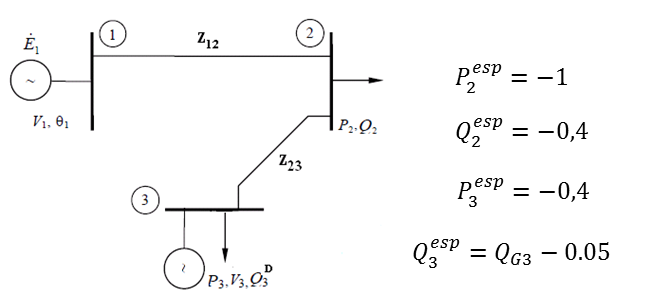
\includegraphics{aula3_10}\protect\caption{\label{fig:aula3_10} Exemplo }
\end{centering}
\end{figure}

\[
P_{1}^{calc}=1,1[1,1(0,33)+V_{2}(-0,33\cos\theta_{2}-3,3\sin\theta_{2})]
\]


\[
Q_{1}^{calc}=1,1[1,1(0,33)+V_{2}(-0,33\sin\theta_{2}-3,3\cos\theta_{2})]
\]


\[
P_{2}^{calc}=V_{2}\cdot[1,1\cdot(-0,33\cdot\cos\theta_{2}+B_{21}\cdot\sin\theta_{2})+V_{2}\cdot(1,706)+1,05\cdot(1,376\cdot\cos\theta_{32}+4,587\cdot\sin\theta_{32})]
\]


\[
Q_{2}^{calc}=V_{2}\cdot[1,1\cdot(1,706\cdot\sin\theta_{2}+7,887\cdot\cos\theta_{2})-V_{2}\cdot(7,887)+1,05\cdot(1,376\cdot\cos\theta_{32}+4,587\cdot\sin\theta_{32})]
\]


\[
P_{3}^{calc}=1,05\cdot[V_{2}\cdot(-1,376\cdot\cos\theta_{32}+4,587\cdot\sin\theta_{32})+1,05\cdot(1,376)]
\]


\[
Q_{3}^{calc}=1,05\cdot[V_{2}\cdot(-1,376\cdot\sin\theta_{32}+4,587\cdot\cos\theta_{32})-1,05\cdot(4,587)]
\]
Considerando:
\[
F(x)={ \begin{matrix} [\triangle { P }_{ 1 } & \triangle { P }_{ 3 } & \triangle { P }_{ 3 } & \triangle { Q }_{ 1 } & \triangle { Q }_{ 2 } & \triangle { Q }_{ 3 }] \end{matrix} }_{ 6 }^{ T }
\]
\[
x={ \begin{matrix} [\theta _{ 1 } & \theta _{ 2 } & \theta _{ 3 } & V_{ 1 } & V_{ 2 } & V_{ 3 }] \end{matrix} }_{ 6 }^{ T }
\]
\[
F(x)={ \begin{matrix} [\triangle { P }_{ 3 } & \triangle { P }_{ 3 } & \triangle { Q }_{ 2 } \end{matrix}] }_{ 3 }^{ T }
\]
\[
x={ \begin{matrix} [\theta _{ 2 } & \theta _{ 3 } & V_{ 2 }] \end{matrix} }_{ 3 }^{ T }
\]
\begin{enumerate}
\item Arbitrar uma condição inicial $(x^{(i)}=x^{(0)})$ e fixar $i=0$;
\[
{ x }^{ (0) }={ \begin{matrix} [0 & 0 & 1 \end{matrix}] }_{ 3 }^{ T }
\]
\item Calcular $F(x^{(i)})$ e verificar a convergência. Se $\max| F(x^{(i)})|\leq \varepsilon$,
parar.
\item Linearizar a função em torno de $(F(x^{(i)}),x^{(i)})$ e igualar
a função a zero para estabelecer o passo $(\varDelta x^{(i)}=x^{(i+1)}-x^{(i)})$
e o novo ponto $(x^{(i+1)})$.
\[
F(x)=F(x^{(i)})+[J(x^{(i)}]\cdot(x^{(i+1)}-x^{(i)})=0
\]
 
\[
x^{(i+1)}=x^{(i)}+[J(x^{(i)}]^{-1}\cdot F(x^{(i)})
\]


Para solucionar o problema proposto devemos determinar a matriz jacobiana:
\begin{figure}[H]
\begin{centering}
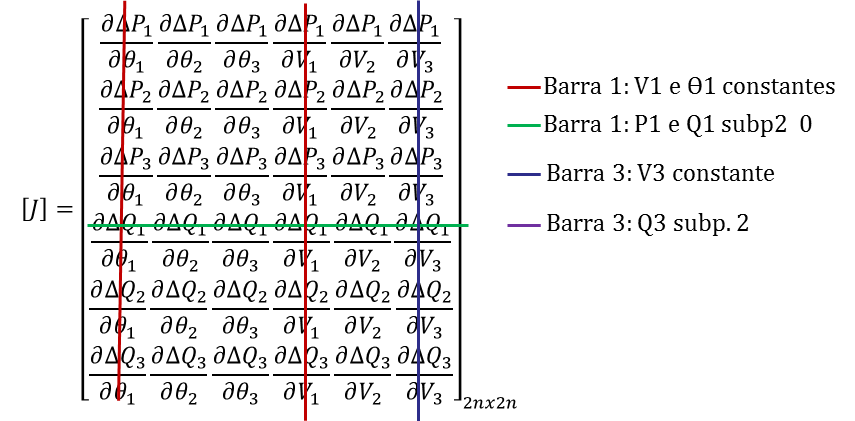
\includegraphics{aula3_11}\protect\caption{\label{fig:aula3_11} Matriz jacobiana do exemplo }
\end{centering}
\end{figure}
O problema apresentado faz com que, para o subproblema 1:
\[
F(x)={ \begin{matrix} [\triangle { P }_{ 3 } & \triangle { P }_{ 3 } & \triangle { Q }_{ 2 } \end{matrix}] }_{ 3 }^{ T }
\]
\[
x={ \begin{matrix} [\theta _{ 2 } & \theta _{ 3 } & V_{ 2 }] \end{matrix} }_{ 3 }^{ T }
\]
Barra 1: $V\theta$(slack bus)

Barra 2: $PQ$(barra de carga)

Barra 3: $PV$(barra de controle de tensão)
\item Fazer $i=i+1$ e voltar ao passo 2.

\end{enumerate}

A matriz Jacobiana par ao problema proposto fica:

\begin{figure}[H]
\begin{centering}
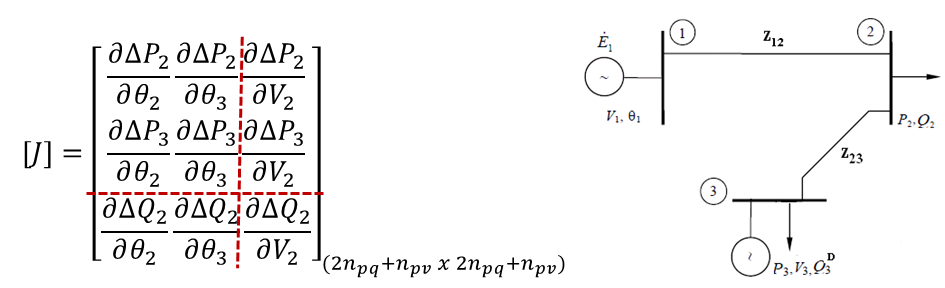
\includegraphics{aula3_12}\protect\caption{\label{fig:aula3_12} Matriz jacobiana }
\end{centering}
\end{figure}
Sendo

$n_{pq}$-Número de barras $PQ$;

$n_{pv}$-Número de barras $PV$;
De outra forma:
\begin{figure}[H]
\begin{centering}
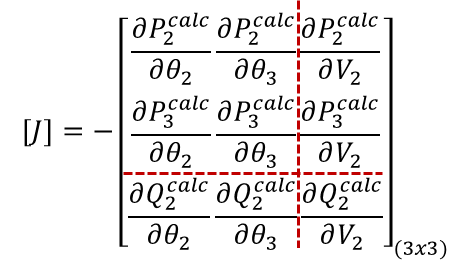
\includegraphics{aula3_13}\protect\caption{\label{fig:aula3_13} Matriz jacobiana }
\end{centering}
\end{figure}

A solução do problema proposto depois de quatro iterações:

\begin{tabular}{|c|c|c|c|c|c|}
\hline 
Barras & V (p.u) & $P_{G}$ & $P_{D}$ & $Q_{G}$ & $Q_{D}$\tabularnewline
\hline 
\hline 
1 (Ref.) ($\theta_{1}=0)$ & 1,1 & - & 0 & - & 0\tabularnewline
\hline 
2 (PQ) & - & 0 & 1 & 0 & 0,4\tabularnewline
\hline 
3 (PQV) & 1,05 & 0,6 & 0,2 & - & 0,05\tabularnewline
\hline 
\end{tabular}
\begin{figure}[H]
\begin{centering}
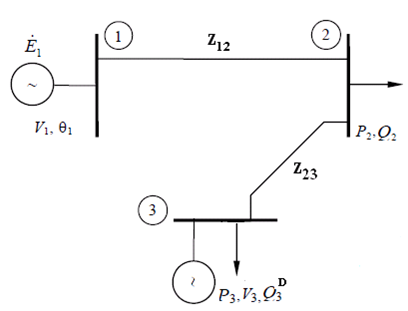
\includegraphics{aula3_14}\protect\caption{\label{fig:aula3_14} Exemplo }
\end{centering}
\end{figure}

$z_{12}=-0,03+0,3j$

$z_{23}=-0,06+0,2j$
\[
{ x }^{ (4) }={ \begin{matrix} { [\theta _{ 2 } }^{ (4) } & { \theta _{ 3 } }^{ (4) } & { V_{ 2 } }^{ (4) }] \end{matrix} }_{ \quad }^{ T }={ \begin{matrix} [-0,1616\quad rad & -0,0958\quad rad & 0,993] \end{matrix} }_{ \quad }^{ T }\quad 
\]
\[
{ x }^{ (4) }={ \begin{matrix} { [\theta _{ 2 } }^{ (4) } & { \theta _{ 3 } }^{ (4) } & { V_{ 2 } }^{ (4) }] \end{matrix} }_{ \quad }^{ T }={ \begin{matrix} [-{ 9,263 }^{ \circ } & { -0,0958 }^{ \circ } & 0,993] \end{matrix} }_{ \quad }^{ T }\quad 
\]

$\varepsilon=0,000001$







